
\documentclass{article}
\usepackage[utf8]{inputenc}
\usepackage{times}
\usepackage[titletoc]{appendix}
\usepackage{graphicx}
\usepackage{lineno}
\usepackage{multirow}
\usepackage[english]{babel}
\usepackage{typearea} 
\usepackage{amssymb}
\usepackage{amsfonts}
\usepackage{amsmath}
\usepackage{enumerate}
\usepackage{mathtools}
\usepackage{graphicx}
\usepackage{wrapfig}
\usepackage{lscape}
\usepackage{rotating}
\usepackage[numbers]{natbib}
\usepackage[colorinlistoftodos]{todonotes}
\newcommand{\Fig}[1]{Figure~\ref{fig:#1}}

\renewcommand{\baselinestretch}{1.5}
\newcommand{\bbar}[1]{\overline{#1}}

\newcommand\scalemath[2]{\scalebox{#1}{\mbox{\ensuremath{\displaystyle #2}}}}
\renewcommand{\familydefault}{\sfdefault}

\usepackage[font={small},labelfont={bf},justification=justified,margin=0.5cm]{caption}

\renewcommand{\thesection}{}
\renewcommand{\thesubsection}{\arabic{section}.\arabic{subsection}}

\usepackage{color}
         \definecolor{darkred}{rgb}{0.9,0,0}
%         \definecolor{darkgreen}{rgb}{0,0.5,0}
         \definecolor{darkblue}{rgb}{0,0,0.75}
%         \definecolor{magenta}{rgb}{0,0,0.75}
\newcommand{\hhone}{(H,H,1)}
\newcommand{\hhtwo}{(H,H,2)}
\newcommand{\hsone}{(H,S,1)}
\newcommand{\hstwo}{(H,S,2)}
\newcommand{\shone}{(S,H,1)}
\newcommand{\shtwo}{(S,H,2)}
\newcommand{\ssone}{(S,S,1)}
\newcommand{\sstwo}{(S,S,2)}

\newcommand{\hhstar}{(H,H,$\star$)}


\usepackage{hyperref}
\definecolor{darkgreen}{rgb}{0.1,0.6,0.3}
\definecolor{darkred}{rgb}{0.6,0.3,0.1}
\hypersetup{
    colorlinks=true,       % false: boxed links; true: colored links
    linkcolor=blue,          % color of internal links (change box color with linkbordercolor)
    citecolor=darkgreen,        % color of links to bibliography
    filecolor=magenta,      % color of file links
    urlcolor= black           % color of external links
}


% remove this before we submit...
\definecolor{greenie}{rgb}{0.1,0.62,0.0}
\definecolor{orange}{rgb}{0.9,0.3,0.0}
\definecolor{deepblue}{rgb}{0.0,0.0,0.7}
\newcommand{\cha}[1]{\textcolor{darkgreen}{(#1)}}


\title{\vspace*{-22mm}\bf Title}
%\author{Chaitanya S. Gokhale$^{1}$, Joseph Bulbulia$^{2,3}$, Marcus Frean$^{4}$\\
%\normalsize $^1$Research Group for Theoretical Models of Eco-evolutionary Dynamics\\
%\normalsize Department of Evolutionary Theory, \\
%\normalsize Max-Planck Institute for Evolutionary Biology, 24306 Pl\"{o}n, Germany, \\
%\normalsize $^2$School of Humanities, Faculty of Arts, University of Auckland, New Zealand \\
%\normalsize $^3$Max Planck Institute for the Science of Human History, Jena, Germany \\
%\normalsize $^4$School of Engineering and Computer Science, \\
%\normalsize Victoria University of Wellington, New Zealand
%}


\date{}

\begin{document}



\linenumbers
\maketitle

\begin{abstract}
% Suggest we set this up differently:
Abstract stuff
\end{abstract}


\noindent
Keywords: 


\tableofcontents

\section{Introduction}
gwbniwbwnijb


%\textbf{Collective cooperation and resource dynamics}.
%

\section{Deterministic dynamics}
\subsection{Replicator Dynamics}

\subsubsection{Two player games with two strategies}

Replicator dynamics is the core idea of evolutionary dynamics. Replicator dynamics determines how the frequency of different strategies in a population changes over time.
We can analyze the equation used to determine replicator dynamics mathematically.
Let's take the frequency of $A$ and $B$ strategies are $x_A$ and $x_B$ and the fitness of each strategy is $f_A$ and $f_B$. It is a two-player game so we can say, $ x_A+x_B=1 $. We can write two differential equations using the above information
\begin{align}
\frac{dx_A}{dt} = x_A(f_A - \bar{f}) \nonumber \\
\frac{dx_B}{dt} = x_B(f_B - \bar{f}) \label{eq:1}
\end{align}

Now to keep the average fitness of the population constant, we can write an equation,
\begin{align}
\bar{f}= (x_Af_A+x_Bf_B)\label{eq:2}
\end{align} 
also, we can write the previously mentioned equation as $x_B=1-x_A$.
Now, we can substitute this $x_B$ value into the equation \ref{eq:2}, after substituting, we get the undermentioned equation.
\begin{align}
\bar{f}={x_Af_A+ (1-x_A)f_B}\label{eq:3}
\end{align}
Now let's substitute the equation \ref{eq:3} into the equation \ref{eq:1}
\begin{align}
&dx_A/dt=x_A[f_A-(x_Af_A+(1-x_A)f_B)] \nonumber\\
          &=x_A[f_A-x_Af_A-f_B+x_af_B] \nonumber\\
          &=x_A[(1-x_A)f_A-(1-x_A)f_B] \nonumber\\
          &=x_A(1-x_A)(f_A-f_B) \nonumber
\end{align} .
This is for a two-player population. If we have $n$ population, we can denote the equation of replicator dynamics as,
\[dx_i/dt=x_i[f_i(x)-\bar{f}]\]
where $i=1,2,3.....(n-1)$

To proceed with the replicator dynamics, we must understand simplex as the next step.
Simplex is a tool in evolutionary dynamics that helps us understand and visualize how a system evolved through an evolutionary process. We can denote this for $(n-1)$ strategies. But for simplicity, we took a two-player ($n=2$) homogenous process in which for $A$, $x_A=1$ and $x_B=0$, or the same goes for $B$, where, $x_A=0$ and $x_B=1$.
It will represent a line between points $A$ and $B$, with the midpoint being $x_A=x_B=0.5$. 
For another example, if we homogeneously use $ n=3$, it will represent an equatorial triangle, and the midpoint of the simplex will be $x_A=x_B=x_C=1/3$.
In population genetics, this simplex is known as the de Finetti diagram.
Let's get back to the replicator dynamics now, Let's write the payoff matrix,\\
\[
\begin{array}{c|cc}
    & A & B \\
    \hline
  A & (a_1) & (a_0) \\
  B & (b_1) & (b_0)
\end{array}
\]
We can write the replicator dynamics as,\\
\[dx_A/dt=x_A(1-x_A)(f_A-f_B)\],
What does this equation tell us? 
We can understand that the rate of change of the frequency of a certain type with time depends on the fitness, average fitness of the population, and frequency. From this understanding, we can state that if $f_i(x)-\bar{f}>0$ then the frequency of this type will increase over time, and if $f_i(x)-\bar{f}<0$, the frequency of the type will decrease over time.
If we make the change of strategy $A$ constant over time , which means $dx_A/dt=0$ then we can write the replicator dynamics equation as,
\[x_A(1-x_A)(f_A-f_B)=0\]
Now, if we try to find the certain under which $dx_A/dt$ will be $0$.
We will have three certain conditions,
\[x=0,x=1\] and \[f_A=f_B\]
$x=0$ and $x=1$ will be the two end points of a single line simplex and the joining point for the frequency graph and the dynamics of this frequency depends on the values of $f_A$ and $f_B$. If $f_A>f_B$ then the curve will be over the $0$ if $f_A<f_B$ then the curve will be under $0$, and for the condition $f_A=f_B$, it will make a straight line between the $0$ and $1$\cite{Bishop1976}.We can calculate the particular frequency where the strategy $A$ becomes abundant from rare or rare from abundant. We can calculate the particular turning point or saturation point frequency using this $f_A=f_B$ equation.\\
Let's take this frequency as $ x^*$.
As we know, $f_A=f_B$
So we can write,
\[xa_0+(1-x)a_1=xb_0+(1-x)b_1\]
\[x(a_0-a_1)+a_1=x(b_0-b_1)+b_1\]
\[x(a_0-a_1-b_0+b_1)=b_1-a_1\]
\[x=\frac{b_1-a_1}{a_0-a_1-b_0+b_1}\]
We can write the $x$ as the above-mentioned frequency as $x^*$
\[x^*=\frac{b_1-a_1}{a_0-a_1-b_0+b_1}\]


For a visual representation of this graph, we can plot this equation for different values of $f_A$ and $f_B$ using Python.
\begin{figure}[h]
        \centering
        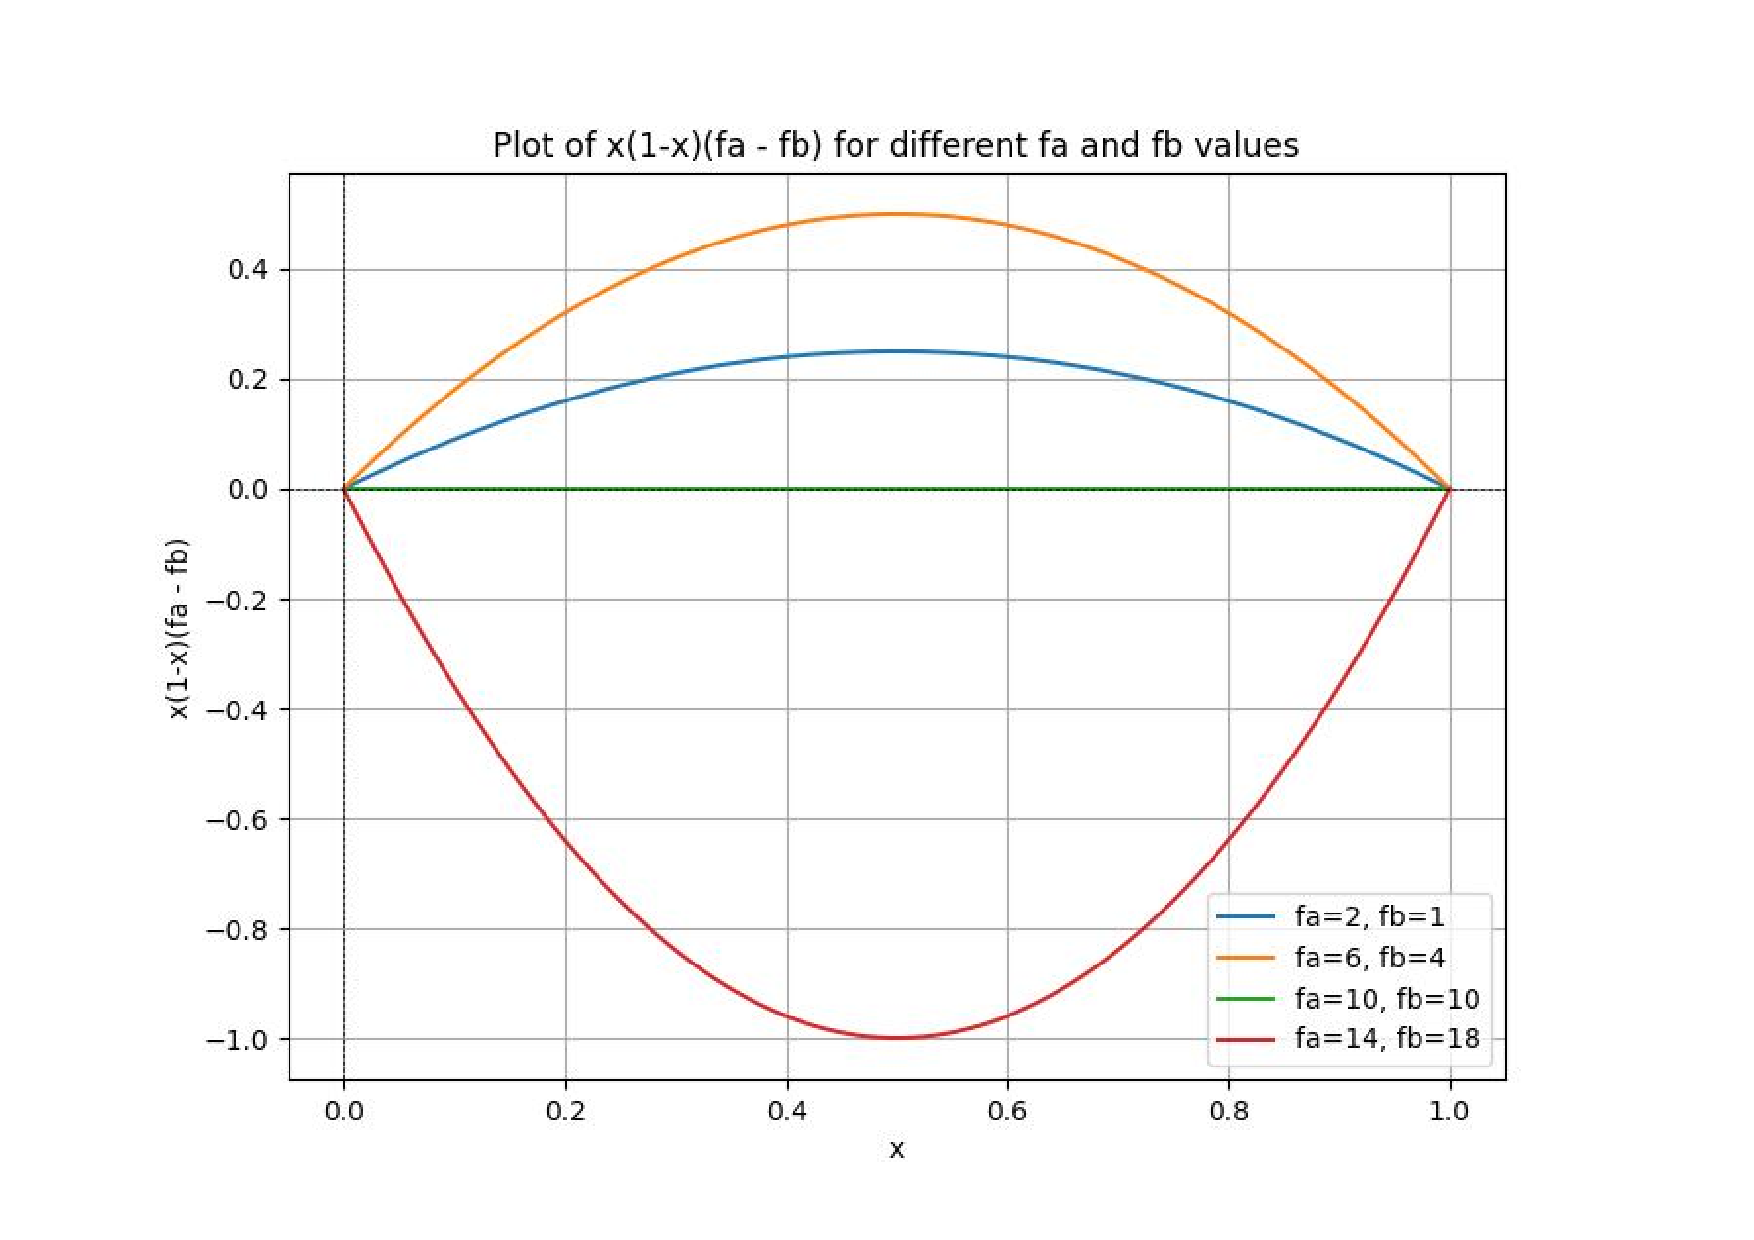
\includegraphics[width=0.5\linewidth]{Figure_1.pdf}
        \label{fig:Visualization of $x_a(1-x_a)(f_a-f_b)=0$}
    \end{figure}
We can get different conditions from this equation and graph. 
(1) Dominance: Where any of the two strategies will be dominant over another, means, for example, if $f_A>f_B$, that strategy $A$ will be dominant over strategy $B$. It will be possible if the $a_1>b_1$ and $a_0>b_0$ where $a_1,a_0,b_1,b_0$ are the payoffs of a payoff matrix of a two-player game.\\
(2) Co-existence: It happens when one of the two strategies is rare and has an advantage for that. For example, if strategy $A$ is rare, then $f_A>f_B$. if $a$ becomes abundant, it will lose its advantage, so the inequality will be  $f_A<f_B$, and while becoming abundant strategy from rare strategy, there will be a saturation point and the equation will $f_A=f_B$. In this scenario, the player should play the rare strategy.It will be possible if the $a_1<b_1$ and $a_0>b_0$ where $a_1,a_0,b_1,b_0$ are the payoffs of a payoff matrix of a two-player game.\\
(3) Bi-stability: A condition where all $A$ and $B$ will be stable. It means that a strategy will get an advantage if it is abundant. For example, if strategy $A$ is abundant, then the inequality will be $f_A>f_B$, and if it becomes rare, then the inequality will be $f_A<f_B$, and there will be a saturation point when $f_A=f_B$. For this condition, the player should play the strategy its opponent is playing.It will be possible if the $a_1>b_1$ and $a_0<b_0$ where $a_1,a_0,b_1,b_0$ are the payoffs of a payoff matrix of a two-player game.\\
(4) Neutrality: Now, we have one condition in which both strategies will have the same impact. It does not depend on the change in the strategy. The equation for this strategy will be $f_A=f_B$.It will be possible if the $a_1=b_1$ and $a_0=b_0$ where $a_1,a_0,b_1,b_0$ are the payoffs of a payoff matrix of a two-player game.\cite{Gokhale2011}.\\
Now, based on the above explained process of replicator dynamics for two players with two strategies, we will explore some games and find their equilibrium point.\\

\textbf{Prisoner's dilemma}
\newline
The prisoner's dilemma is a fundamental game in the game theory, which represents that two rational individuals might not cooperate, even if it benefits mutually.\\
The game goes as two prisoners ($A$ player and $B$ player) are arrested by a policeman and offered some deals separately.\\
There will be mainly three conditions,\\
One, if both prisoners cooperate, they will get equal and moderate amount of sentence.\\
Two, if one prisoner defects, the defector will get no sentence, but the cooperator gets a longer sentence.\\
Three, if both players defect, both will get a lower and equal sentence.\\
Let's try to write the payoff matrix,
\[
\begin{array}{c|cc}
    & \text{Cooperate (C)} & \text{Defect (D)} \\
    \hline
    \text{Cooperate (C)} & (R,R) = (3,3) & (S,T) = (0,5) \\
    \text{Defect (D)} & (T,S) = (5,0) & (P,P) = (1,1)
\end{array}
\]
The general and standard condition for prisoner' dilemma is $T>R>P>S$.\\
As mentioned in the replicator dynamics section, there will be three points where the value of $dx/dt$ will be $0$. The three conditions are $x=0$, it means only defectors, and $x=1$, which means only cooperators; these two are boundary points.\\
The internal equilibrium will fulfil the condition of $f_C=f_D$.Let's find the equilibrium point by putting the payoff values\\
\[xR+(1-x)S= xT+(1-x)P\]
\[x^*=\frac{P-S}{(R-S)+(P-T)}\]
Let's put the values of payoffs,
\[x^*=\frac{1-0}{(3-0)+(1-5)}= -1\]
Since the boundary points are ${0,1}$, there can not exist any internal equilibrium valued $-1$. This states that the entire system will transition to full defection $(x=0)$ over time.
We can plot the graph using Python for the Prisoner's dilemma dynamics.\\

\textbf{Chicken Game}
\newline
In this game, two players( player $a$ and player $b$)are driving towards each other in a single pathway. There are two options for the players,\\
Swerve(C)- Avoided collision but appeared weak.\\
Stay (D)- Stay driving toward each other, hoping the opponent will swerve.\\
We can write three conditions based on this: \\
One, if both swerves, they will not face collision, but there will be a small loss.\\
Two, if one swerves and one stays, the one who stays will have a win, and one who swerves will face loss.\\
Three, if both stay, they both stay, they'll have a huge loss.\\
We can write the payoff matrix with actual payoffs, which follow the standard condition, $a_1<b_1$ and $a_0>b_0$.\\
\[
\begin{array}{c|cc}
   & \text{Swerve (C)} & \text{Stay (D)} \\
  \hline
  \text{Swerve (C)} & (-c) = (-3) & (b) = (4) \\
  \text{Stay (D)} & (0) = (0) & (\frac{b}{2}) = (2) \\
\end{array}
\]
As we know, there will be three points where the value of $dx/dt$ will be $0$. The three conditions are $x=0$, it means only defectors, and $x=1$, which means only cooperators; these two are boundary points.\\
The internal equilibrium will fulfil the condition of $f_C=f_D$.Let's find the equilibrium point by putting the payoff values.\\
\begin{align}
&x(b)+(1-x)(-c)=x(b/2)+(1-x)(0)\nonumber\\
&4x-3+3x=2x \nonumber\\
&x=\frac{3}{5} \nonumber\\
&x^*=\frac{3}{5} \nonumber
\end{align}
This implies that over time, $3/5$ of the population will stay and $2/5$ of the population will swerve respectively.It implies the condition of co-existence\\
Let's try to plot it.\\
\textbf{Stag Hunt Game}
\newline
Stag hunt game is a classical example of game theory for understanding social dilemma and the interplay between risk and trust.
In this game, two players are hunting in a forest. They have two choices,Cooperate(C) with each other and hunt stag or Independently hunt hare(D).\\
We can write three conditions based on this,\\
One,If they both cooperate and hunt stag, they will get the highest payoff.\\
Two, If One goes for the stag hunt and the other one hunts hare, the one who hunts stag will get nothing and the one who hunts hare will get a lower payoff.\\
Three, If they both defect and independently hunt hare, they will get a lower payoff.\\
We can write the payoff matrix using actual values, which follow the conditions of $a_1>b_1$ and $a_0<b_0$.
\[
\begin{array}{c|cc}
   & \text{Cooperate (C)} & \text{Defect (D)} \\
  \hline
  \text{Cooperate (C)} & (S,S) = (4,4) & (S,H) = (0,3) \\
  \text{Defect (D)} & (H,S) = (3,0) & (H,H) = (3,3) \\
\end{array}
\]
As we know, there will be three points where the value of $dx/dt$ will be $0$. The three conditions are $x=0$, it means only defectors, and $x=1$, which means only cooperators; these two are boundary points.\\
The internal equilibrium will fulfil the condition of $f_C=f_D$.Let's find the equilibrium point by putting the payoff values.\\
\begin{align}
&x(0)+(1-x)(4)=x(3)+(1-x)(3) \nonumber\\
&4-4x=3x+3-3x \nonumber\\
&4x=3 \nonumber\\
&x= \frac{3}{4} \nonumber\\
&x^*=\frac{3}{4}\nonumber
\end{align}
Over time,it implies that  $3/4$ of the population will hunt stag and the $1/4$ of the population will hunt hare.\\

\subsubsection{Two player games with multiple strategies}
In the previous subsection, we analysed two player games with two strategies, now we are going to analyse two player games with multiple strategies.For better understanding of this particular problem, let's take a biological example, strains of \textit{Escherichia coli} are competing for resources available on the media. $K$ strain is the killer strain which produces toxin that will out-compete strain $S$. So, having toxin or not are the two strategies, we can write this using two strategy payoff matrix but there can be another possibility, where strain $R$ is resistant to the toxin but pay the cost for resistance. SO, the scenario now changed completely, now the payoff matrix will be $3 \times 3$. This study was carried out by\cite{Kerr2002}\cite{Czaran2002}
Now, in a population there will be multiple strategies.So, we have to write the replicator dyanmics in $(n-1)$ dimensional simplex.For that we need $n\times n$ payoff matrix.
\[
\begin{array}{c@{}c}
   & \begin{array}{cccc} 1 & 2 & \dots & n \end{array} \\ 
   \begin{array}{c} 
       1 \\ 
       2 \\ 
       \vdots \\ 
       n 
   \end{array} 
   & 
   \begin{pmatrix}
       a_{1,1} & a_{1,2} & \dots & a_{1,n} \\
       a_{2,1} & a_{2,2} & \dots & a_{2,n} \\
       \vdots & \vdots & \ddots & \vdots \\
       a_{n,1} & a_{n,2} & \dots & a_{n,n}
   \end{pmatrix}
\end{array}
\]
This is a two player game,here $a_{1,2}$ means player $A$ playing strategy $1$ agaisnt the strategy $2$ of palyer $B$ so we can write the equation using replicator dyanmics,
\[dx_i/dt=x_i[f_i(x)-\bar{f}]\]
We can derive the average fitness of a strategy $i$ from this equation,
\[f_i(x)=a_{i,1}x_1+a_{i,2}x_2+.....+a_{i,n}x_n\]
We can write this equation as,
\[f_i(x)=\sum_{j=1}^{n}a_{i,j}x_j\]
and the average fitness of a population is given by
\[\bar{f}=x_1f_1+x_2f_2+.....+x_nf_n= \sum_{i=1}^{n}x_if_i \]\\
\textbf{Rock Paper Scissor Game}
\newline
Rock paper scissor game is a game in which there are $n=3$ strategies for each player. There are mainly three conditions,\\
One,if rock, paper and scissor meet respectively with rock, paper and scissor, the payoff will be zero. \\
Two, if rock meets with scissor and paper with rock and scissor with paper , they will get the highest payoff.\\
Three, if the rock meets with paper and paper with scissor and scissor with rock, they will get the lowest payoff.\\
Let's try to write the payoff matrix.\\
\[
A =
\begin{pmatrix}
  & R & S & P \\
R & 0 & 1 & -1 \\
S & -1 & 0 & 1 \\
P & 1 & -1 & 0
\end{pmatrix}
\]
Let's write the average payoff,\\
For Rock,
\begin{align}
f_R &= (0)p_R + (1)p_S + (-1)p_P \nonumber\\
f_R &= p_S - p_P \nonumber
\end{align}
For Scissor,
\begin{align}
f_S &= (-1)p_R + (0)p_S + (1)p_P \nonumber\\
f_S &= p_P - p_R \nonumber
\end{align}
For Paper,
\begin{align}
f_P &= (1)p_R + (-1)p_S + (0)p_P \nonumber\\
f_P &= p_R - p_S \nonumber
\end{align}
Now the mathematical condition for finding the internal equilibrium is,$f_R=f_S=f_P$.
\begin{align}
f_R &=f_S \nonumber\\
p_S-p_P &=p_P-p_R \nonumber\\
p_P &= \frac{p_S+p_R}{2} \label{eq:4}
\end{align}
\begin{align}
f_S &=f_P \nonumber\\
p_P-p_R &=p_R-p_S \nonumber\\
p_R &= \frac{p_P+p_S}{2} \label{eq:5}
\end{align}
\begin{align}
f_R &=f_P \nonumber\\
p_S-p_P &=p_R-p_S \nonumber\\
p_S &= \frac{p_R+p_P}{2} \label{eq:6}
\end{align}
After solving the equations \ref{eq:4}, \ref{eq:5}, \ref{eq:6}, we can say that probability of using these strategies are in symmetry because each probability can be expressed by other two probabilities and the structure of equation remains the same.\\
So the internal equilibrium will be $p_R=p_S=p_P=\frac{1}{3}$




\section{Probabilistic Dynamics}
\subsection{Stochastic Process and Finite Population}
\subsubsection{Two players with two strategies}
In the previous subsection, we used an infinite population for the deterministic approach\cite{Hofbauer2003}. Now, we will proceed with a finite population. There are mainly two reasons to use a finite population: first, it is realistic, and second, it is a natural way to introduce randomness into the replicator dynamics\cite{Altrock2010}.
Now, we can consider the finite population of a specific game as $N$.Let's assume there are two strategies $a$ and $b$. Frequencies for $a$ and $b$ are $i$ and $(N-i)$. We can write the payoff matrix according to this specification,
\[
\begin{array}{c|cc}
    & a & b \\
    \hline
  a & (a_1) & (a_0) \\
  b & (b_1) & (b_0)
\end{array}
\]
Now we can denote the average payoff of $a$ and $b$ strategies as $\pi_a$ and $\pi_b$.
\[\pi_a=\frac{i-1}{N-1}a_1 + \frac{N-i}{N-1}a_0\]
\[\pi_b=\frac {i}{N-1}b_1 + \frac{N-i-1}{N-1}b_0\]
Now, a question can arise, why are we using $i-1$ instead of $i$? We have to understand that instead of an infinitely large population, we are using a real finite population and for that, we have to remove the particular individual who is observing or analysing this situation. So we use $i-1$.
In the previous work, we used fitness directly related to payoff. But in the actual population, we introduce a tunable parameter similar to the fitness which controls the game.
Nowak et al.\cite{Nowak2004} introduced this tunable parameter as selection intensity. Because for some situations or equations, we can know the particular relation between the fitness and payoff but for most of the cases, we don't know the particular relation, we can just create a hypothesis.
\[f_i=1-w+w\pi_i\]
where $w$ selection intensity and $\pi_i$ is the payoff. The value of $w$ is bound by  $0$ and $1$. If the value is $0$ then $f_i=1$, we can deduce from this equation that for every value of $i$, we will face neutrality, and if the value is $1$, we will have $f_i=\pi_i$, now it suggests that the game payoff controls the fitness.
Now, we can move to the part of the evolutionary dynamics where, for the finite population, there's randomness involved in the population. So, we will go for the stochastic processes.
For these stochastic processes, we will focus on the Moran process. It consists of two events: birth and death. For the birth, one subject is chosen randomly, and it produces it's identical copy, and for the death process again, one random subject is chosen from the population and eliminated. It means by introducing randomness with the birth-death process now this theory can change the population with each time step, and for $N$ steps it will control a generation \cite{Moran1962}
There are three mathematical equations that we can derive from this theory: (1) The number of $a$ individuals increases by 1; (2) the number of $a$ individuals decreases by 1; (3)The number of $a$ individuals remains neutral.\\
For the (1) scenario, we can write:
\[T_i^+=\frac{if_a}{if_a+(N-i)f_b}\frac{N-i}{N}\]
For the (2) scenario, we can write:
\[T_i^-=\frac{(N-i)f_a}{if_a+(N-i)f_b}\frac{i}{N}\]
For the (3) scenario, we can write:
\[1-T_i^+-T_i^-\]
Now what can we deduce from these equations?\\
From the (1) equation, we can say that $a$ numbered individuals can increase only when an $a$ individual is chosen for birth and an $b$ individual is chosen for death.\\
From the (2) equation, we can say that the number of $a$ decreases cause, an $a$ individual is chosen for death and an $b$ individual is chosen for birth.\\
From the (3) equation, we can deduce that no one is chosen for the birth or death process, so there's a neutrality.\\
Now, let us jump to the fixation probability.\\
In genetics, we often ask a question related to the invasion of a gene, how can the gene invade another gene, and how it affect the another gene's population?
After understanding the transition probability and moran processes, we can now form a question based on the previous mentioned topic. In population of $j$ numbered $a$ individuals and $(N-j)$ numbered $b$ individuals, what is the probability that the whole population will become of $a$ individuals?
This is known as the fixation probability of $j$ numbered $a$ individuals.We can denote this fixation probability as $\rho(j)$.
Since, fixation is an absorbing state, so if all of the population once becomes $a$, it can not be revert. We can try to write a probability balance equation.
\[\rho(j)=T_i^+\rho_a(j+1)+(1-T_i^+-T_i^-)\rho_a(j)+T_i^-\rho_a(j-1)\]
We can derive This discrete stochastic process using the absorbing phenomenon of Markov chain processes.
Let's solve this equation.
\[\rho_a(j)-\rho_a(j-1)=\frac{T_i^-}{T_i^+}(\rho_a(j+1)-\rho_a(j))\]
\[T_i^++(\rho_a(j)-\rho_a(j-1)=T_i^-(\rho_a(j+1)-\rho_a(j)\]
\[T_i^+\rho_a(j)-T_i^+\rho_a(j-1)=T_i^-\rho_a(j+1)-T_i^-\rho_a(j)\]
\[\rho_a(j+1)=\frac{\rho_a(j)(T_i^+ + T_i^-)-T_i^+\rho_a(j+1)}{T_i^-}\]
 Now, let's write the equation.\\
 $Ratio_j=R_j=\frac{T_i^-}{T_i^+}= \frac{(N-j)f_b}{jf_a}$
 Let's substitute the value of $R_j$
 \[\rho_a(j+1)={\rho_a(j)(1+R_j)-R_j\rho_a(j-1)}\]
 Let's solve this equation by putting some real values,\\
 We get this underwritten equation by putting the value of $j=1$,
 \[\rho_a(2)= \rho_a(1)(1+R_1)-R_1\rho_a(0)\]
 Let's put $j=2$.
 \[\rho_a(3)=\rho_a(2)(1+R_2)-R_2\rho_a(1)\]
 Let's substitute the value of $\rho_a(2)$
 \[\rho_a(3)=\rho_a(1)(1+R_1)(1+R_2)-\rho_a(1)\]
 \[\rho_a(3)=\rho_a(1)((1+R_1)(1+R_2)-1)\]
 Now we can write a general equation based on this.
 \[\rho_a(j)=\left[1+\sum_{m=1}^{j-1}\prod_{i=1}{m}R_i \right] \rho_a(1)\]
 Since we know that $j=N$, and fixation is guaranteed means $\rho_a(N)=1$
 \[1=\left[1+\sum_{m=1}^{N-1}\prod_{i=1}^{m} R_i\right]\rho_a(1)\]
 \[\rho_a(1)=\frac{1}{1+\sum_{m=1}^{N-1}\prod_{i=1}^{m}R_i}\]
 We can use this above-mentioned equation when we are proceeding with just $1$ player population.
 So, we can write the final fixation probability equation as,
 \[\rho(j)=\frac{1+\sum_{m=1}^{j-1}\prod_{i=1}^{m}R_i}{1+\sum_{m=1}^{N-1}\prod_{i=1}^{m}R_i}\]
 If we consider a neutral drift, where $f_a=f_b$, then we can write the equation as, $\rho_a={j}/{N}$.
 If we observe the neutral drift with a single individual, we can write $\rho_a=1/N$\cite{Traulsen2006}\\

 We can calculate the fixation probability for strategy $b$ as $\rho_b$. $1$ $b$ individual reaches fixation is equal to the $N-1$ $a$ individuals fails to reach fixation.
\[\rho_b=1-\rho_a(N-1)\]
\[=1-\frac{1 + \sum_{m=1}^{N-2} \prod_{i=1}^{m} R_i}{1 + \sum_{m=1}^{N-1} \prod_{i=1}^{m} R_i}\]
\[=\frac{1}{1+\sum_{m=1}^{N-1}\prod_{i=1}^{m}R_i}(\prod_{i=1}^{N-1}R_i)\]
\[=\rho_a(\prod_{i=1}^{N-1}R_i)\]


\cha{I like the use of $R_j$ as it makes some of the notations quite nice! Next, I would try to simulate the process by starting with a single player of a second strategy and $N-1$ of the first. See what happens when you change the selection intensity for the same three games you would have explored in the two-player two strategy case. On the graphs, plot the analytical expression starting with a single mutant as a line and plot the simulation results as dots.}





\section{Discussion}


\textbf{Code availability}.
Appropriate computer code describing the model is available at 
\texttt{ REDACTED for review}.% {\url{https://github.com/tecoevo/beliefs}}.

\section{Acknowledgements}
\texttt{ REDACTED for review}.% {\url{https://github.com/tecoevo/beliefs}}.


\bibliographystyle{naturemag}
\bibliography{references.bib}

\renewcommand{\theequation}{SI.\arabic{equation}}
\setcounter{equation}{0}

\renewcommand{\thefigure}{SI.\arabic{figure}}
\setcounter{figure}{0}

\section{Supplementary material}


\subsection{Analysis of the simple system}




\end{document}
